\zexternaldocument{evaluatie}
\zexternaldocument{inleiding}
\zexternaldocument{imp}

\chapter{Naar het automatisch toevoegen van vereisten en afhankelijkheden}
\label{sec:afhankelijkheden}
Configuratiebeheergereedschappen die gebruik maken van vereisten en afhankelijkheden reduceren het aantal fouten tijdens het uitrolproces en zorgen voor een snellere convergentie naar de gewenste toestand.
Dit hoofdstuk introduceert enkele heuristieken die proberen extra vereisten en afhankelijkheden toe te voegen aan het configuratiemodel.

De heuristieken zijn deels ge\"inspireerd door situaties die in de inleiding al voorgesteld werden. 
Secties \ref{sec:bestanden_en_mappen} beschrijft een heuristiek die garandeert dat bestanden en mappen altijd in juiste volgorde gecre\"eerd worden.
Sectie \ref{sec:stacks} en \ref{sec:namen} introduceren heuristieken die vereisten toevoegen tussen logisch samenhorende resources.
De heuristieken uit secties \ref{sec:relaties} en \ref{sec:vereisten_uit_afhankelijkheden} werken samen om relaties om te zetten in vereisten om zo een effici\"entere volgorde opleggen aan het uitrolproces.  

\section{Vereisten tussen bestanden en mappen}
\label{sec:bestanden_en_mappen}
Deze heuristiek garandeert dat elk bestand pas aangemaakt wordt na zijn bovenliggende map.
Als namelijk een omgekeerde volgorde gehanteerd wordt mislukt het uitrollen van het bestand.
Figuur \ref{fig:file_dir_dep} geeft hiervan een visuele voorstelling.

\begin{figure}
    \begin{center}
    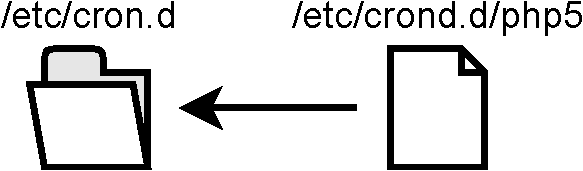
\includegraphics[width=0.6\textwidth]{images/file_dir_dep.pdf}
    \caption{Grafische voorstelling van de afhankelijkheid tussen een bestand en zijn bovenliggende folder}
    \label{fig:file_dir_dep}
    \end{center}
\end{figure}

Het algoritme dat hiervoor gebruikt wordt ziet eruit als volgt (pseudocode):
\begin{minipage}{\textwidth}
\begin{lstlisting}[language=Python]
for file in host.resources:
    for dir in host.resources:
        if get_directory(file.path) == dir.path:
            file.requires.add(dir)
\end{lstlisting}
\end{minipage}

Als de map niet vermeld wordt in het model wordt deze ook niet toegevoegd omdat dit ongewenste gevolgen kan hebben.
Dit zou namelijk fouten verbergen die de gebruiker kan maken bij het opstellen van het model.
Als hij bijvoorbeeld een bestand plaatst in de configuratiemap van een pakket (bvb ``/etc/ldap'') maar het pakket zelf (``ldap'') vergeet toe te voegen aan het model krijgt hij geen foutmelding.
De map wordt namelijk automatisch aangemaakt.


\section{Vereisten tussen services, packages en configuratiebestanden}
\label{sec:stacks}
Net zoals bij bestanden en mappen zijn er voorwaarden voor het correct uitrollen van packages, services en hun eventuele configuratiebestanden:
een service kan niet starten als zijn package niet ge\"installeerd is en zal niet correct werken zonder een aangepast configuratiebestand.
De verzameling van een service, het pakket dat die service installeert en de configuratiebestanden wordt vanaf nu een stack genoemd.
Een schematische voorstelling van de onderlinge vereisten bnnen een stack is te vinden op figuur \ref{fig:stack}.

\begin{figure}[h]
    \begin{center}
    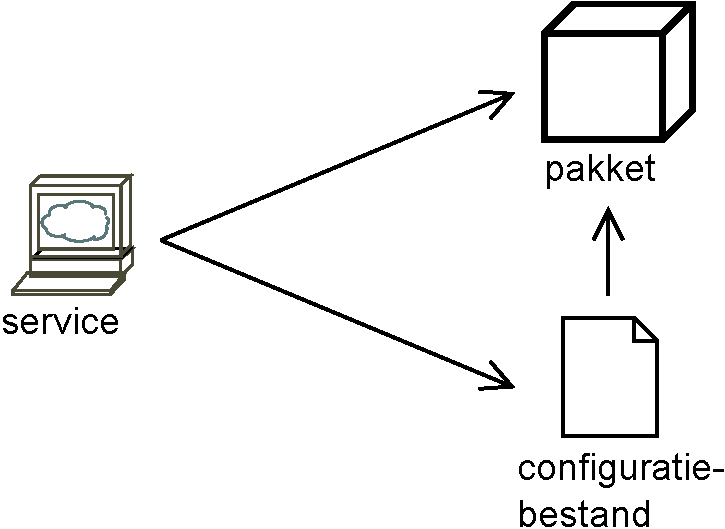
\includegraphics[width=0.6\textwidth]{images/stack.pdf}
    \caption{Grafische voorstelling van de onderlinge vereisten van packages, services en configuratiebestanden binnen een stack}
    \label{fig:stack}
    \end{center}
\end{figure}

Een eerste aanpak om de correcte afhankelijkheden te introduceren is alle pakketten en bestanden een vereiste maken van alle services en alle pakketten een vereiste van alle bestanden.
De configuratiebestanden mogen pas geplaatst worden nadat de packages ge\"installeerd zijn omdat anders het aangepast configuratiebestand overschreven wordt.
Dit introduceert uiteraard veel afhankelijkheden die niet overeenstemmen met de werkelijkheid maar ze maken daardoor het resultaat van het uitrolproces niet fout.
Als het model maar \'e\'en stack bevat voegt de heuristiek geen enkele overbodige vereiste toe, bij twee stacks zes overbodige vereisten, bij drie stacks 27,\ldots
Een algoritme in pseudocode ziet er uit als volgt:

\begin{minipage}{\textwidth}
\begin{lstlisting}[language=Python]
for service in host.resources:
    for file in host.resources:
        service.requires.add(file)
    for package in host.resources:
        service.requires.add(package)
for file in host.resources:
    for package in host.resources:
        file.requires.add(package)
\end{lstlisting}
\end{minipage}

Deze heuristiek resulteert in een soort batchuitvoering waarbij de CMS  eerst alle pakketten installeert, dan alle (configuratie)bestanden aanmaakt en uiteindelijk alle services opstart.

De volgende aanpak gebruikt meer info uit het model en resulteert in minder overbodige afhankelijkheden.
In het model worden bestanden, pakketten en services die deel uitmaken van een geheel gegroepeerd in een ``implementatie''.
Een voorbeeld is de MySQL server:

\begin{minipage}{\textwidth}
\begin{lstlisting}
implementation mysql:
    pkg = std::Package(host= host, name= "mysql-server", state= "installed")
    svc = std::Service(host= host, name= "mysqld", state= "running", onboot= true)

    config= std::ConfigFile(host= host, path= "/etc/my.cnf", content= template("mysql/my.cnf.tmpl"), requires= pkg, reload= true)
    conf_dir= std::Directory(host= host, path= "/etc/mysql.conf.d", owner= "root", group= "root", mode= 755)

    dblist= std::ConfigFile(host= host, path= "/etc/sysconfig/mysql", reload= true, content= template("mysql/databases.tmpl"))
end
\end{lstlisting}
\end{minipage}

Alles dat staat tussen ``implementation mysql'' en ``end'' is gedefini\"eerd binnen \'e\'enzelfde scope.
Deze heuristiek zoekt verzamelingen van packages en services die binnen \'e\'enzelfde scope gedefini\"eerd zijn en stelt de correcte afhankelijkheden op tussen enkel die groep resources.
De aanwezigheid van files is optioneel: sommige services hebben geen aangepast configuratiebestand nodig.

\begin{minipage}{\textwidth}
\begin{lstlisting}
srv_stacks = []
for resource in resources:
    same_scope = [res in resources where res.scope == resources.scope]
    if same_scope.contains(services) and same_scope.contains(packages):
        srv_stacks.add(same_scope)

for stack in srv_stacks:
    for service in stack:
        for file in stack:
            service.requires.add(file)
        for package in stack:
            service.requires.add(package)
    for file in stack:
        for package in stack:
            file.requires.add(package)
\end{lstlisting}
\end{minipage}

Deze heuristiek voegt geen overbodige vereisten toe.
Resultaten van het gebruik van deze heuristiek staan in sectie \ref{sec:stacks_eval}.

\section{Vereisten tussen resources met gelijkaardige naam}
\label{sec:namen}
De laatste heuristiek heeft een gelijkaardige doel als de vorige: vereisten opstellen tussen samenhorende resources.
In plaats van te werken binnen een scope zoekt deze heuristiek naar resources met een gelijkaardige naam.

Om de vereisten tussen services en de bijhorende pakketten en bestanden op te stellen wordt de naam van de service gebruikt.

Om de vereisten tussen pakketten en de configuratiebestanden op te stellen worden twee aanpassingen gedaan aan de naam van het pakket.
Allereerst worden alle cijfers uit de naam van het pakket verwijderd.
Daarna wordt alles na een splitsingsteken verwijderd.
Zo stelt de heuristiek ook afhankelijkheden op tussen bijvoorbeeld het pakket ``cassandra12'' en het configuratiebestand ``/etc/cassandra.conf'' of het pakket ``openssh-server'' en ``/etc/openssh.conf''. 
\todo{waarom niet gewoon naam van service gebruiken? Truukjes zijn dan niet nodig.}
\begin{minipage}{\textwidth}
\begin{lstlisting}
for service in host.resources:
    similar_resources = []
    for file in host.items:
        if file.name.contains(service.name):
            service.requires.add(file)
    for package in host.items:
        if package.name.contains(service.name):
            service.requires.add(package)

for package in host.resources:
    name = remove_digits(package.name)
    name = name.split("-")[0]
    for file in host.items:
        if file.name.contains(service.name):
            package.requires.add(file)
\end{lstlisting}
\end{minipage}

\section{Afhankelijkheden door relaties}
\label{sec:relaties}
IMP laat toe relaties tussen concepten te modelleren.
Een voorbeeldrelatie is de volgende:
\begin{lstlisting}
BaseClient clients [0:] -- [0:] BaseServer servers
\end{lstlisting}
Deze betekent dat een BaseClient nul of meerdere BaseServers nodig heeft, en omgekeerd.
Een ander voorbeeld is 
\begin{lstlisting}
Host host [1] -- [0:] File files
\end{lstlisting}
Dit betekent dat een Host nul of meerdere files kan bevatten\todo{ander woord zoeken}, maar dat elke File op maximaal \'e\'en Host kan uitgerold worden.
De heuristiek leidt hieruit af dat een File niet kan bestaan zonder een host en het dus nodig is dat eerst de Host wordt uitgerold voordat de File wordt aaangemaakt.

Algemeen kan men besluiten dat elke relatie waar de ene kant een multipliciteit van [0] of [0:] heeft en de andere kant multipliciteit [n] of [n:] de eerste entiteit afhankelijk is van de tweede.
De code voor deze heuristiek ziet er uit als volgt:

\begin{minipage}{\textwidth}
\begin{lstlisting}
for lib in model.get_scopes():
    for concept in lib.variables():
        if concept.hasattr(relation)
            if concept.relation.low == 0 and concept.relation.end == 1:
                concept.relation.depends = True
\end{lstlisting}
\end{minipage}

Als enkel deze heuristiek gebruikt wordt zal IMP niets veranderen aan het uitrolproces.
IMP doet zelf niets met de gedefini\"eerde relaties.
De extra informatie kan wel gebruikt worden door andere heuristieken.
Een voorbeeld hiervan is deze hieronder (sectie \ref{sec:vereisten_uit_afhankelijkheden}) die afhankelijke relaties omzet in vereisten.

\section{Vereisten door afhankelijkheden}
\label{sec:vereisten_uit_afhankelijkheden}
Deze heuristiek heeft als doel afhankelijke relaties om te zetten in een concrete vereiste tussen resources.
Samengestelde entiteiten zoals een webserver bestaan uit verschillende resources: configuratiebestanden, pakketten en services.
Als een entiteit afhankelijk is van een andere betekent dat dat hij zijn volledige functionaliteit niet kan aanbieden als de andere entiteit nog niet volledig uitgerold is.
Het aanbieden van functionaliteit gebeurt door services, niet door de aanwezigheid van bestanden of pakketten.
Een afhankelijkheid tussen twee entiteiten kan dus gereduceert worden tot een vereiste tussen de services van de twee entiteiten.

Deze heuristiek zoekt naar afhankelijke relaties en voegt de gepaste vereisten toe tussen de services die in relatie staan met elkaar.
In pseudocode ziet dit er uit als volgt:

\begin{minipage}{\textwidth}
\begin{lstlisting}
for lib in model:
    for concept in lib.variables():
        concept_services = get_services(concept)
        if concept_services is not None:
            for relation in concept.get_attributes():
                if relation.depends: #afhankelijke relatie
                    for instance in concept.values: #Voor elke instantie v/h concept
                        req_concepts = relation.end
                        req_resources = []
                        for req_concept in req_concepts:
                                for srv in get_services(req_concept):
                                    req_resources.add(srv)
                        if req_resources is not None: 
                            for service in concept_services:
                                for req_res in req_resources:
                                    service.requires.add(req_res)
\end{lstlisting}
\end{minipage}

Het is belangrijk dat deze heuristiek wordt opgeroepen na deze van sectie \ref{sec:relaties}, daar worden namelijk extra afhankelijke relaties opgesteld die hier kunnen gebruikt worden.

\section{Besluit van dit hoofdstuk}


